% !TEX program = xelatex
\documentclass{beamer}
\usefonttheme[onlymath]{serif}
\setbeamerfont{footnote}{size=\tiny}

% use multiple languages
%% ---- allow CJK usage ---- %%
\usepackage[CJKspace]{xeCJK} % this should be called before Polyglossia
\setCJKmainfont{Noto Serif CJK TC}
\setCJKsansfont{Noto Sans CJK TC}
\setCJKmonofont{Noto Sans Mono CJK TC}
% \setCJKmainfont{Noto Serif JP}
% \setCJKsansfont{Noto Sans JP}
% \setCJKmonofont{Noto Sans Mono CJK JP}

%% ---- ตั้งค่าให้ตัดคำภาษาไทย ---- %%
\XeTeXlinebreaklocale "th"
\XeTeXlinebreakskip = 0pt plus 0pt % เพิ่มความกว้างเว้นวรรคให้ความยาวแต่ละบรรทัดเท่ากัน

%% ---- font settings ---- %%
\usepackage{fontspec}
\defaultfontfeatures{Mapping=tex-text} % map LaTeX formating, e.g., ``'', to match the current font
% To change the main font, uncomment one of the below command.
% \setmainfont{TeX Gyre Termes} % Free Times
% \setsansfont{TeX Gyre Heros} % Free Helvetica
% \setmonofont{TeX Gyre Cursor} % Free Courier
\newfontfamily{\thaifont}[Scale=MatchUppercase,Mapping=textext]{Laksaman} % ตั้งฟอนต์หลักภาษาไทย
\newenvironment{thailang}{\thaifont}{} % create environment for Thai language
\usepackage[Latin,Thai]{ucharclasses} % ตั้งค่าให้ใช้ "thailang" environment เฉพาะ string ที่เป็น Unicode ภาษาไทย
\setTransitionTo{Thai}{\begin{thailang}}
\setTransitionFrom{Thai}{\end{thailang}}

%% ---- spacing between lines ---- %%
\usepackage{setspace}
% \singlespacing % default setting
% \onehalfspacing % recommend using this for Thai language

%% ---- using alphabatic language ---- %%
\usepackage{polyglossia}
\setdefaultlanguage{english} % it is preferrable to set English as the main language, since the numeric system is compatible with most LaTeX features such as 'enumerate' and so on
\setotherlanguages{thai}

\AtBeginDocument\captionsthai % allow captions to be in Thai


%% ---- Title page details ---- %%
\title[]{A time-dependent central core model and a schematic model for passive mechanism}
\author[C. Sint]{Chanoknun Sintavanuruk 
% \\ (ชนกนันท์ สินธวานุรักษ์; 馬予棟) \inst{1} 
% \and author2 \inst{2}
}
% \institute[shortinst]{\inst{1} affiliation 
% % \and \inst{2} affiliation for author2
% }
\date{\today}

% preambles for Beamer

%% ---- math packages ---- %%
\usepackage{amsmath}
\usepackage{amssymb}
\usepackage{bm} % same functionality as \mathbf{} but for greek letters
\numberwithin{equation}{section} % equation numbers are formatted as <#Section>.<#eq in the section>
\usepackage{cancel}
\renewcommand\CancelColor{\color{red}}

%% ---- define math environment ---- %%
\usepackage{amsthm}

%% ---- hyperref settings ---- %%
% \usepackage{hyperref} % Beamer already has hyperref by default
\usepackage{url}
\usepackage{cite}
\usepackage{natbib}
\usepackage{bibentry}
\usepackage{xcolor}
\hypersetup{
    colorlinks,
    linkcolor={red!50!black},
    citecolor={blue!50!black},
    urlcolor={blue!80!black}
    }

%% ---- misc. ---- %%
\usepackage{mhchem} % use chemistry notation
\newcommand\scalemath[2]{\scalebox{#1}{\mbox{\ensuremath{\displaystyle #2}}}} % scale display math environment
\usepackage{lipsum}
\usepackage{metalogo} % for extended LaTeX logo such as XeTeX
\usepackage{subcaption} % allowing subfigure environment
% \usepackage[section]{placeins} % ensure floats do not go into the next section and allow the use of \FloatBarrier
\usepackage{graphicx} % allow cropping and rotating images

%% ---- Theme choice ---- %%
\usetheme{metropolis}
% \usetheme{Berkeley}
% \usecolortheme{beaver}
% \usecolortheme{dove}
% \usecolortheme{spruce}
% \logo{\large \XeTeX{}}

%% ---- show TOC after sections ---- %%
% \AtBeginSection[]
% {
%     \begin{frame}
%         \frametitle{Outline}
%         \tableofcontents[currentsection]
%     \end{frame}
%     }

%% ---- Show notes ---- %%
\usepackage{pgfpages}
% \setbeameroption{show notes}
% \setbeameroption{show notes on second screen=right}
% for working around text color bug when using XeLaTeX
\makeatletter 
\def\beamer@framenotesbegin{% at beginning of slide
     \usebeamercolor[fg]{normal text}
      \gdef\beamer@noteitems{}% 
      \gdef\beamer@notes{}% 
}
\makeatother

%% ---- page numbers ---- %%
% \setbeamertemplate{page number in head/foot}[totalframenumber]\setbeamertemplate{navigation symbols}{\footnotesize\usebeamertemplate{page number in head/foot}}

%% ---- figure numbering ---- %%
\setbeamertemplate{caption}[numbered]

\setbeamerfont{caption}{size=\scriptsize}

\begin{document}
% Title page frame
\begin{frame}
    \titlepage 
\end{frame}
% Remove logo from the next slides
% \logo{}

% Outline frame
\begin{frame}{Outline}
    \tableofcontents
\end{frame}

\section{Time-dependent model}

\subsection{Model equations}

\begin{frame}{Compartments}
    Multiphasic medulla on the domain $(0,L)$ (superficial $\to$ deep).
    \begin{enumerate}
        \item Central core ($k=0$)
        \item Descending tubule ($k=\mathrm{D}$)
        \item Ascending tubule ($k=\mathrm{A}$)
        \item Collecting tubule ($k=\mathrm{C}$)
    \end{enumerate}
\end{frame}

\begin{frame}{Cross-sectional areas}
    Cross-sectional areas $\alpha_k$ ($\text{cm}^2$) satisfy
    \begin{equation}\label{eq:vol_conserv}
        \sum_k \alpha_k = \alpha_*
    \end{equation}
        where $\alpha_*:(0,L)\to \mathbb{R}_+$ is the fixed medullary cross-sectional area.
    \pause
    \begin{align}\label{eq:volume_dynamics}
        \frac{\partial \alpha_k}{\partial t} + \frac{\partial}{\partial x}\left( \alpha_k u_k \right) &= -\beta_kw_k,\quad k=\mathrm{D},\mathrm{A},\mathrm{C},\\
        \frac{\partial \alpha_0}{\partial t} + \frac{\partial }{\partial x}\left( \alpha_0 u_0 \right) &= \sum_{k=\mathrm{D},\mathrm{A},\mathrm{C}} \beta_kw_k.
    \end{align}
    $u_k$: axial flow \textit{velocity} (cm/s); $w_k$: transmural flux (cm/s); $\beta_k$: total tubular circumferences (cm)
\end{frame}

\begin{frame}{Water flow and transport}
    Poiseuille's equation:
    \begin{equation}
        % \frac{\rho_k u_k}{\alpha_k} = -\frac{\partial p_k}{\partial x},\quad k=0,\mathrm{D},\mathrm{A},\mathrm{C},
        \frac{8\pi\eta_k u_k}{\alpha_k} = -\frac{\partial p_k}{\partial x},\quad k=0,\mathrm{D},\mathrm{A},\mathrm{C},
    \end{equation}
    $\eta_k$: viscosity (mmHg$\cdot$s), $p_k$: pressure (mmHg).
    \pause

    Water transport:
    \begin{equation}
        w_k := \zeta_k\left( \psi_k - \psi_0 \right),\quad  k=\mathrm{D},\mathrm{A},\mathrm{C}
    \end{equation}
    % \pause
    % Osmotic pressure:
    \begin{equation}
        \left. \begin{aligned}
            \psi_k&:=p_k - \pi_k,\\
            \pi_k&:= RT\left( 2c_\mathrm{s}^k+c_\mathrm{u}^k\right),
        \end{aligned} \right\}
        \quad k=0,\mathrm{D},\mathrm{A},\mathrm{C}.
    \end{equation}
    $\zeta_k$: water permeability (mmHg$\cdot$s); $c_i^k$: concentration (mmol/$\text{cm}^3$)
\end{frame}

\begin{frame}{Pressure-compliance relationship}
    Given tubular compliance $\nu_k$ ($\text{mmHg}^{-1}$), we assume
    \begin{equation}
        \nu_k(p_k - p_0) = \frac{\alpha_k}{\bar{\alpha}_k} - 1,\quad k=\mathrm{D},\mathrm{A},\mathrm{C}.
    \end{equation}
    Note that $p_0$ is determined by the medullary volume conservation (\ref{eq:vol_conserv}).
\end{frame}

\begin{frame}{Solute dynamics}
    \begin{align}\label{eq:solute_dynamics}
        \frac{\partial}{\partial t}\left( \alpha_k c_i^k \right)&=-\frac{\partial}{\partial x} f_i^k - \beta_kg_i^k,\quad k=\mathrm{D},\mathrm{A},\mathrm{C},\\
        \frac{\partial}{\partial t}\left( \alpha_0 c_i^0 \right)&=-\frac{\partial}{\partial x} f_i^0 + \sum_{k=\mathrm{D},\mathrm{A},\mathrm{C}} \beta_k g_i^k,
    \end{align}
    $f_i^k$: Axial solute flow (mmol/s):
    \begin{equation}
        f_i^k := \alpha_k\left( -D_i^k\frac{\partial c_i^k}{\partial x}+u_kc_i^k \right),\quad k=0,\mathrm{D},\mathrm{A},\mathrm{C}.
    \end{equation}
    $D_i^k$: diffusion coefficient ($\text{cm}^2$/s).

    $g_i^k$: transmural solute flux (mmol/$\text{cm}^2\cdot$s),
\end{frame}

\begin{frame}{solute transport}
    $g_i^k$: transmural solute flux (mmol/$\text{cm}^2\cdot$s), (adapted from \cite{Stephenson1987,Stephenson1989}):
    \begin{equation}
        g_i^k := j_i^k+h_i^k,\quad k=\mathrm{D},\mathrm{A},\mathrm{C},
    \end{equation}
    \begin{equation}
        % \left. \begin{aligned}
        %     j_i^k &= \gamma_i^k\left( \mu_i^k - \mu_i^0 \right)\\
        %     \mu_i^k &:= RT\ln c_i^k,\quad 
        % \end{aligned} \right\}\quad k=0,\mathrm{D},\mathrm{A},\mathrm{C}
        j_i^k = \gamma_i^k\left( c_i^k - c_i^0 \right),\quad k=0,\mathrm{D},\mathrm{A},\mathrm{C}.
    \end{equation}
    $\gamma_i^k$: solute permeability (cm/s).

    $h_i^k$: active transport:
    \begin{equation}
        h_\mathrm{s}^\mathrm{A} = \begin{cases}
            \frac{{h}_\mathrm{s,max}^\mathrm{A}}{1+{M}/{c}_\mathrm{s}^\mathrm{A}}\quad &\text{in}\quad (0,\frac{L}{3})\\
            0\quad &\text{in}\quad [\frac{L}{3},L),
        \end{cases}
    \end{equation}
    where $M$ is the Michaelis-Menten constant.
\end{frame}

\begin{frame}{Boundary condition: central core}
    No flux at the bottom:
    \begin{align}
        u_0(t,L) &= 0,\\ 
        f_i^0(t,L)&=0,\quad i=\mathrm{s},\mathrm{u}.
    \end{align}
    Dirichlet boundary at the cortico-medullary junction:
    \begin{align}
        p_0(t,0) &= P_\mathrm{v}(t),\\ 
        c_i^0(t,0) &= c_i^\mathrm{v}(t).
    \end{align}
\end{frame}

\begin{frame}{Boundary condition: descending tubule}
    Input from the PCT:
    \begin{align}
        (\alpha_\mathrm{D} u_\mathrm{D})(t,0) &= F_\mathrm{PCT}(t),\\
        % f_i^\mathrm{D}(t,0) &= (\alpha_\mathrm{D}u_\mathrm{D}c_i^\mathrm{D})(t,0),\quad i=\mathrm{s,u}\\
        c_i^\mathrm{D}(t,0) &= c_{i}^{\mathrm{PCT}}(t),\quad i=\mathrm{s,u},
    \end{align}
    Tip of the loop of Henle:
    \begin{align}
        (\alpha_\mathrm{D}u_\mathrm{D}+\alpha_\mathrm{A}u_\mathrm{A})(t,L) &= 0,\\
        \quad\left( f_i^\mathrm{D}+f_i^\mathrm{A} \right)(t,L) &= 0,\\
        p_\mathrm{D}(t,L)&= p_{\mathrm{A}}(t,L),\\ 
        c_i^\mathrm{D}(t,L) &=c_i^\mathrm{A}(t,L)
    \end{align}
\end{frame}

\begin{frame}{Boundary condition: modification by distal tubules}
    Assumption: salt from the ascending tubule is further reabsorbed so that only a fraction of $q\in (0,1)$ are left at the collecting tubule; formally,
    \begin{align}
        \left( f_{\mathrm{u}}^\mathrm{A}+f_\mathrm{u}^\mathrm{C} \right)(t,0) &= 0,\\
        \left( qf_{\mathrm{s}}^\mathrm{A}+f_\mathrm{s}^\mathrm{C} \right)(t,0) &= 0.
    \end{align}
    Further, we assume that 
    \begin{align}
        % (\alpha_\mathrm{A}u_\mathrm{A}+\alpha_\mathrm{C}u_\mathrm{C})(t,0) &= 0,\\
        % \quad\left( f_i^\mathrm{A}+f_i^\mathrm{C} \right)(t,0) &= 0,\\
        p_\mathrm{A}(t,0)&= p_{\mathrm{C}}(t,0),\\ 
        % c_i^\mathrm{A}(t,0) &=c_i^\mathrm{C}(t,0),
        % \frac{\partial c_i^\mathrm{A}}{\partial x}(t,0)&= 0,\quad i = \mathrm{s},\mathrm{u},
        f_i^\mathrm{A}(t,L) &= (\alpha_\mathrm{A}  u_\mathrm{A}  c_i^\mathrm{A})(t,L),\quad i = \mathrm{s},\mathrm{u},\\ 
        (2c_\mathrm{s}^\mathrm{C}+c_\mathrm{u}^\mathrm{C})(t,0) &=\mathrm{osm}_\mathrm{cortex}(t),
    \end{align}
        where the cortical osmolarity $\mathrm{osm}_\mathrm{cortex}$ is given.
\end{frame}

\begin{frame}{Boundary condition: papillary outflow}
    \begin{align}
        % (\alpha_\mathrm{C} u_\mathrm{C} )(t,L) &= \max\left\{ 0,\frac{p_\mathrm{C} (t,L) - P_{\mathrm{p}} }{R_{\mathrm{p}}}\right\},\\
        p_\mathrm{C} (t,L) &= P_{\mathrm{p}}(t),\\
        f_i^\mathrm{C}(t,L) &= (\alpha_\mathrm{C}  u_\mathrm{C}  c_i^\mathrm{C})(t,L),\quad i=\mathrm{s},\mathrm{u},
    \end{align}
        where $P_\mathrm{p}$ is the papillary pressure.
\end{frame}

% \begin{frame}[Boundary condition: papillary outflow (2/2)]
%     {\color{red} Or we can replace (\ref{eq:no_diff_pap}) by
%     \begin{equation}
%         c_i^\mathrm{C}(t,L) = K*\left( f_i^\mathrm{C}\left( \cdot,L \right) \right)(t)=\int_{\mathbb{R}}K(t-s) f_i^\mathrm{C}(s,L)\,ds,
%     \end{equation}
%     where $K\in L^1(\mathbb{R})$ is non-negative, monotone decreasing in $\mathbb{R}_+$, and $K(t)=0$ for $t<0$.}
% \end{frame}

\subsection{Non-dimensionalization \& numerical simulation}
\begin{frame}{Rescaling}
    Introduce spatial rescaling and advective timescale:
    \begin{equation}
        x = L\hat{x},\quad t = \tau\hat{t},\quad \tau:=\frac{L}{p_*/\rho_*L}=\frac{8\pi\eta_*L^2}{\bar{\alpha}c_*RT}
    \end{equation}
        where the subscript $*$ denotes the typical magnitude of physical quantities; here $p_* = c_*RT$ and $\rho_* = 8\pi\eta_*/\bar{\alpha}$ are those of pressure and hydraulic resistivity with $\bar{\alpha} = \frac{1}{L}\int_0^L\alpha_*(x)\,dx$.

    Unknowns:
    \begin{gather}
        \alpha_k = \bar{\alpha}\hat{\alpha},\quad c_i^k = c_*\hat{c}_i^k,\quad p_k = p_*\hat{p}_k = c_*RT\hat{p}_k.
    \end{gather}    
\end{frame}

\begin{frame}{Dimensionless model}
    \begin{align}
        \frac{\partial \hat{\alpha}_k}{\partial \hat{t}}  + \frac{\partial}{\partial \hat{x}}\left( \hat{\alpha}_k \hat{u}_k \right) &= - \hat{w}_k,\\ \label{eq:nd_1steq}
        \frac{\partial\hat{\alpha}_0}{\partial \hat{t}}+\frac{\partial}{\partial \hat{x}}\left( \hat{\alpha}_0 \hat{u}_0 \right) &=\sum_k \hat{w}_k,\\
        \hat{\nu}_k\left( \hat{p}_k - \hat{p}_0 \right) &= \frac{\hat{\alpha}_k}{\hat{\bar{\alpha}}_k}-1,\\
        \hat{\alpha}_0 + \sum_{k} \hat{\alpha}_k &= \hat{\alpha}_*,\\
        \frac{\partial}{\partial \hat{t}}\left( \hat{\alpha}_k \hat{c}_i^k \right)&=-\frac{\partial}{\partial \hat{x}} \hat{f}_i^k - \hat{g}_i^k,\\
        \frac{\partial}{\partial \hat{t}}\left( \hat{\alpha}_0 \hat{c}_i^0 \right)&=-\frac{\partial}{\partial \hat{x}} \hat{f}_i^0 + \sum_k \hat{g}_i^k,
    \end{align}
\end{frame}

\begin{frame}{Dimensionless flows and transports}
    \begin{align}
        \hat{u}_{k} &:= -\frac{\hat{\alpha}_{k}}{\hat{\rho}_{k}}\frac{\partial \hat{p}_{k}}{\partial \hat{x}},\\
        \hat{f}_i^{k} &:= \hat{\alpha}_{k}\left( -\hat{D}_i^{k} \frac{\partial \hat{c}_i^{k}}{\partial \hat{x}} + \hat{u}_{k}\hat{c}_i^{k} \right),\\
        \hat{w}_k&:= \hat{\zeta}_k\left( \hat{\psi}_k-\hat{\psi}_0 \right),\quad\hat{\psi}_{k} := \hat{p}_{k} - \left(  2\hat{c}_\mathrm{s}^{k}+\hat{c}_\mathrm{u}^{k} \right),\\
        \hat{g}_i^k &:= \hat{j}_i^k+\hat{h}_i^k,\quad \hat{j}_i^k =\hat{\gamma}_i^k(\hat{c}_i^k-\hat{c}_i^0). \label{eq:nd_lasteq}\\
        \hat{h}_\mathrm{s}^\mathrm{A} &= \begin{cases}
            \frac{\hat{h}_\mathrm{s,max}^\mathrm{A}}{1+\hat{M}/\hat{c}_\mathrm{s}^\mathrm{A}}\quad &\text{in}\quad (0,\frac{1}{3})\\
            0\quad &\text{in}\quad [\frac{1}{3},1)
        \end{cases}
    \end{align}
\end{frame}

\begin{frame}{Parameters and boundary conditions}
    Parameters (note that $\beta_k$ is absorbed into $\hat{\zeta}^k_i,\hat{\zeta^k_{\mathrm{w}}}$):
    \begin{gather*}
        % \mathrm{Pe} = \frac{\bar{\alpha}p_*/\rho_*}{D_*},\quad 
        \hat{\rho}_{k} = \frac{8\pi\eta_{k}}{\rho_*},\quad 
        \hat{\nu}_k = p_*\nu_k,\quad \hat{\bar{\alpha}}_{k} = \frac{\bar{\alpha}_{k}}{\bar{\alpha}},\quad \hat{\alpha}_* = \frac{\alpha_*}{\bar{\alpha}}\\
        \hat{D}_i^{k} = \frac{\tau}{L^2}D_i^{k},\quad 
        % \hat{\zeta}_k = \frac{\beta_k c_*L^2}{\bar{\alpha}D_*}\zeta_k,\quad\hat{\gamma}_i^k = \frac{\beta_kRT L^2}{\bar{\alpha}c_* D_*}\gamma_i^k,
        \hat{\zeta}_k = \frac{\beta_k p_*\tau}{\bar{\alpha}}\zeta_k,\quad\hat{\gamma}_i^k = \frac{\beta_kp_*\tau}{\bar{\alpha}c_*^2}\gamma_i^k,\\
        \hat{h}_\mathrm{s}^\mathrm{A} = \frac{\beta_\mathrm{A}\tau}{\bar{\alpha}c_*}h_\mathrm{s}^\mathrm{A},\quad \hat{M} = \frac{M}{c_*}.
    \end{gather*}
    Boundary conditions are the same but with $\hat{\cdot}$ notation where
    \begin{gather*}
        F_\mathrm{PCT} = \frac{\bar{\alpha}L}{\tau}\hat{F}_\mathrm{PCT},\quad
        P_\mathrm{p} = p_*\hat{P}_\mathrm{p},\quad
        P_\mathrm{v} = p_*\hat{P}_\mathrm{v},\\
        c_i^\mathrm{v} = c_*\hat{c}_i^\mathrm{v},\quad \mathrm{osm}_\mathrm{cortex} = c_*\widehat{\mathrm{osm}}_\mathrm{cortex}.
    \end{gather*}

\end{frame}

\begin{frame}{Numerical simulation}
    \begin{itemize}
        \item Approximation: backward difference for time derivatives and central difference for spatial derivatives. Then, use an iterative method.
        \item Most parameters except for $D_i^k$ when $k\neq 0$, $\eta_k$, $P_\mathrm{v}$, $P_\mathrm{p}$, $\nu_k$, $q$ are available in \cite{Stephenson1987,Stephenson1989} which uses transfusion data in rabbit; these 6 will be chosen empirically.
        \item The simulated solution appears to converge to a steady state.
    \end{itemize}
\end{frame}

\begin{frame}{Parameters}
    Physical and geometric parameters (take $\bar{\alpha}_k = \pi r^2$, $\beta_k = 2\pi r_k$, $\alpha_* = \sum_k \bar{\alpha}_k$):

    \resizebox{\textwidth}{!}{
    \begin{tabular}{||c c c|c|c|c c c c||} 
        \hline
        $D_\mathrm{s}^0$ & $D_\mathrm{u}^0$ & $D_i^k$, $k\neq 0$ & $\eta_k$ & $\nu_k$ & $r_0$ & $r_\mathrm{D}$ & $r_\mathrm{A}$ & $r_\mathrm{C}$\\
        \hline
        \multicolumn{3}{||c|}{{\tiny($\times 10^{-4}\,\text{cm}^2$/s)}} & {\tiny (cP $\approx 7.5\times 10^{-6}$ mmHg$\cdot$s)} & {\tiny ($\text{mmHg}^{-1}$)} & \multicolumn{4}{|c||}{{\tiny ($\times 10^{-3}$ cm)}}\\
        \hline\hline
        2.5 & 2 & 0.15 & 0.6915 & 0.0517 & 2.5 & 0.8 & 1 & 1.2 \\ %[1ex] 
        \hline
       \end{tabular}       
    }
    
    Transport parameters:

    \resizebox{\textwidth}{!}{
    \begin{tabular}{||c c c|c c c|c c c|c c||} 
        \hline
        $\zeta_\mathrm{D}$ & $\zeta_\mathrm{A}$ & $\zeta_{\mathrm{C}}$ &
         $\gamma_\mathrm{s}^\mathrm{D}$ & $\gamma_\mathrm{s}^\mathrm{A}$ & $\gamma_\mathrm{s}^\mathrm{C}$ & 
         $\gamma_\mathrm{u}^\mathrm{D}$ & $\gamma_\mathrm{u}^\mathrm{A}$ & $\gamma_\mathrm{u}^\mathrm{C}$ & $h_{\mathrm{s,max}}^{\mathrm{A}}$ & $M$ \\
        \hline
        \multicolumn{3}{||c|}{{\tiny ($\times 10^{-8}$ cm/mmHg$\cdot$s)}} & \multicolumn{6}{|c|}{{\tiny ($\times 10^{-5}$ cm/s)}} & {\tiny ($\frac{10^{-6}\text{mmol}}{\text{cm}^2\cdot\text{s}}$)} & {\tiny ($\frac{\text{mmol}}{\text{cm}^{3}}$)} \\ %[1ex] 
        \hline\hline
        22.5 & 0 & 3.95 & 1.61 & 6.27 & 0.04 & 1.5 & 0.86 & 0 & 14.2 & 0.15 \\ %[1ex] 
        33.8 & 0 & 3.95 & 1.61 & 26.0 & 0.04 & 1.5 & 6.70 & 0 & 0 &  \\ %[1ex] 
        26.4 & 0 & 3.95 & 1.61 & 26.0 & 0.04 & 1.5 & 6.70 & 1.5 & 0 &  \\ %[1ex] 
        \hline
    \end{tabular}   
    }

\end{frame}

\begin{frame}{Boundary data}
    \begin{tabular}{||c|c c|c c c||} 
        \hline
        $F_\mathrm{PCT}$ & $P_\mathrm{p}$ & $P_\mathrm{v}$ & $c_\mathrm{s}^\mathrm{v}$ & $c_\mathrm{u}^{\mathrm{v}} $ & $\mathrm{osm}_\mathrm{cortex}$ \\
        \hline
        {\tiny ($\times 10^{-7}\text{cm}^{3}$/s)} & \multicolumn{2}{|c|}{{\tiny (mmHg)}} & \multicolumn{3}{|c||}{{\tiny (mmol/L)}}\\
        \hline\hline
        1.67 & 6.4 & 0 & 145 & 5 & 295 \\ %[1ex] 
        \hline
       \end{tabular}       
\end{frame}
    
\begin{frame}{Result}
    
    \begin{figure}
        \centering
        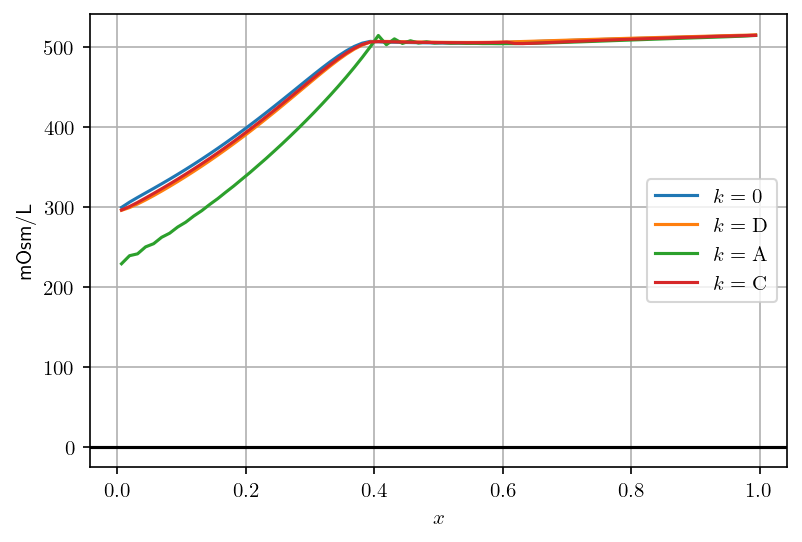
\includegraphics[width=\textwidth]{../results/6-6-2023/osm.png}
    \end{figure}
\end{frame}

\section{Schematic model for passive mechanism}

\begin{frame}{Idea}
    \begin{itemize}
        \item We want to have a clean picture of what makes passive mechanism working.
        \item Derive a schematic model of \textit{inner medulla} based on the common explanation of passive mechanism:
    \end{itemize}
    \begin{alertblock}{Concept of passive mechanism}
        The net water and NaCl reabsorption preceding the inner medulla collecting tubules concentrate the urea enough that it diffuses out in the inner medulla.
        This in turn increases osmolality in the interstitium that drives the water reabsorption from the thin descending limbs, concentrating NaCl in the process.
        NaCl is then passively reabsorbed at the ascending tubule.
    \end{alertblock}
    
\end{frame}

\begin{frame}{Model derivation}
    Consider a steady state of the previous dimensionless model but rescale $\hat{x}\in (0,1)$ to be the \textit{inner medulla} instead (from now on, we omit the $\hat{\cdot}$ notation).
    We further make simplifying assumptions that 
    \begin{itemize}
        \item The descending and ascending tubule urea concentration and the collecting tubule salt concentration are negligible.
        \item Zero salt permeability in the descending tubule.
    \end{itemize}

    
\end{frame}

\begin{frame}{}
    Rewriting $q_k = \alpha_ku_k$, $s_k = c_\mathrm{s}^k$, $u_k = c_\mathrm{u}^k$, $\gamma_s = \gamma_\mathrm{s}^\mathrm{A}$, $\gamma_u = \gamma_\mathrm{u}^\mathrm{C}$, and assuming that $1/\nu_k$ and $D_i^k$ are small, we arrive at the leading order equations:
    \begin{columns}[T]

        \begin{column}{0.5\textwidth}
            \begin{align}
                \frac{dq_\mathrm{D}}{dx} &= -\zeta_\mathrm{D}\left( 2s_0+u_0 - 2s_\mathrm{D} \right) = -w_\mathrm{D},\label{eq:q_D_eq}\\
                \frac{dq_\mathrm{A}}{dx} &= 0,\label{eq:q_A_eq}\\
                \frac{dq_\mathrm{C}}{dx} &= -\zeta_\mathrm{C}\left( 2s_0+u_0 - u_\mathrm{C} \right) = -w_\mathrm{C},\label{eq:q_C_eq}\\
                \frac{dq_0}{dx} &= w_\mathrm{D}+w_\mathrm{C},\label{eq:q_0_eq}
            \end{align}
        \end{column}
        
        \begin{column}{0.5\textwidth}
            \begin{align}
                \frac{d}{dx}(s_\mathrm{D}q_\mathrm{D}) &= 0,\label{eq:s_D_eq}\\
                \frac{d}{dx}(s_\mathrm{A}q_\mathrm{A}) &= -\gamma_s(s_\mathrm{A} - s_0),\label{eq:s_A_eq}\\
                \frac{d}{dx}(s_\mathrm{0}q_\mathrm{0}) &= \gamma_s(s_\mathrm{A} - s_0),\label{eq:s_0_eq}\\
                \frac{d}{dx}(u_\mathrm{C}q_\mathrm{C}) &= -\gamma_u(u_\mathrm{C} - u_0),\label{eq:u_C_eq}\\
                \frac{d}{dx}(u_\mathrm{0}q_\mathrm{0}) &= \gamma_u(u_\mathrm{C} - u_0).\label{eq:u_0_eq}
            \end{align}
        \end{column}
    
    \end{columns}
    
\end{frame}

\begin{frame}
    9 unknowns: the water flow $q_\mathrm{D},q_\mathrm{A},q_\mathrm{C},q_0$ and the solute concentrations $s_\mathrm{D},s_\mathrm{A},s_0,u_\mathrm{C},u_0$. (Note that in the limit as $1/\nu_k\searrow 0$, $p_k$ are identical.)

    The ODEs are completed with 9 boundary conditions:
    \begin{equation}\label{eq:q_bdry}
        q_\mathrm{D}(0) = \frac{2S}{C},\quad q_\mathrm{A}(1) = -q_\mathrm{D}(1),\quad q_\mathrm{C}(0) = \frac{U}{C},\quad q(1) = 0.
    \end{equation}
    \begin{equation}\label{eq:solute_bdry}
        2s_\mathrm{D}(0) = u_\mathrm{C}(0) = C,
    \end{equation}        
    \begin{align}
        \frac{2S}{C}+q_0(0)+q_\mathrm{A}+\frac{U}{C} &= q_\mathrm{C}(1),\label{eq:w_consv}\\
        S+q_\mathrm{A}(0)s_\mathrm{A}(0)+s_0(0)q_0(0) &= 0,\label{eq:s_consv}\\
        U+u_0(0)q_0(0) &= u_\mathrm{C}(1)q_\mathrm{C}(1).\label{eq:u_consv}
    \end{align}
    The problem can be reduced even further!
\end{frame}

\begin{frame}
    After some tedious calculation, we can explicitly solve for $q_\mathrm{A}$, $q_0$, $s_\mathrm{D}$, $s_0$, $u_0$ in terms of $q_\mathrm{D}$, $q_\mathrm{C}$, $s_\mathrm{A}$, $u_\mathrm{C}$.
    Hence, this problem is equivalent to
    \begin{align}
        \frac{dq_\mathrm{D}}{dx} &= -\zeta_\mathrm{D}\left( 2s_0+u_0-\frac{2S}{q_\mathrm{D}} \right) \label{eq:sys_q_D}\\
        \frac{ds_\mathrm{A}}{dx} &= -\frac{\gamma_s}{q_\mathrm{A}}(s_\mathrm{A} - s_0),\label{eq:sys_s}\\
        \frac{dq_\mathrm{C}}{dx} &= -\zeta_\mathrm{C}(2s_0+u_0-u_\mathrm{C}),\label{eq:sys_q_C}\\
        \frac{du_\mathrm{C}}{dx} &= \frac{1}{q_\mathrm{C}}\left(\zeta_\mathrm{C}u_\mathrm{C}(2 s_0+u_0 - u_\mathrm{C})- \gamma_u(u_\mathrm{C} - u_0)\right),\label{eq:sys_u}
    \end{align}
        with boundary conditions
    \begin{equation}\label{eq:sys_bdry}
        % \begin{gathered}
            % s_\mathrm{A}(0) = s_0(0) + s_\mathrm{A}(1)\left( 1-\frac{s_0(0)}{S} \left( \frac{2S+U}{C} - q_\mathrm{C}(1) \right) \right),\\
            q_\mathrm{D}(0) = \frac{2S}{C},\quad
            s_\mathrm{A}(1) = S/q_\mathrm{D}(1),\quad
             q_\mathrm{C}(0) = \frac{U}{C},\quad u_\mathrm{C}(0) = C.
        % \end{gathered}
    \end{equation}
        % where $q_\mathrm{A} = -q_\mathrm{D}(1)$, and $s_0,u_0$ are given by
        % \begin{equation}\label{eq:su}
        %     s_0 = \frac{S-s_\mathrm{A}q_\mathrm{D}(1)}{q_\mathrm{D} - q_\mathrm{D}(1)+q_\mathrm{C} - q_\mathrm{C}(1)},\quad u_0 = \frac{u_\mathrm{C}q_\mathrm{C} - u_\mathrm{C}(1)q_\mathrm{C}(1)}{q_\mathrm{D} - q_\mathrm{D}(1)+q_\mathrm{C} - q_\mathrm{C}(1)}.
        % \end{equation}
\end{frame}

\begin{frame}{Exploring passive mechanism}
    The system of ODEs is approximated using central difference scheme, then solved using an iterative method.
    \begin{figure}
        \centering
        \begin{subfigure}{0.5\textwidth}
            \centering
            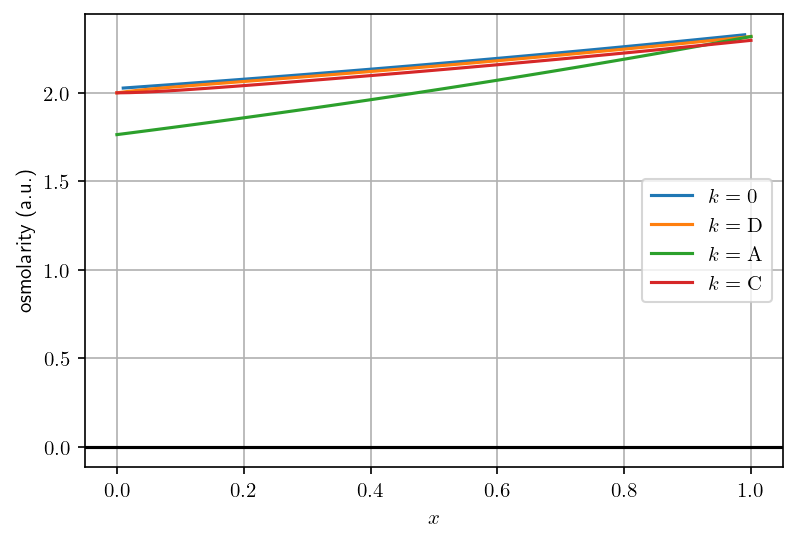
\includegraphics[width=\linewidth]{../results/7-20-2023/osm_low_solute_perm.png}
            \caption{$\gamma_u = \gamma_s = 0.1$}
            \label{fig:low_sol_perm}
            \vspace*{4mm}
        \end{subfigure}%
        \begin{subfigure}{0.5\textwidth}
            \centering
            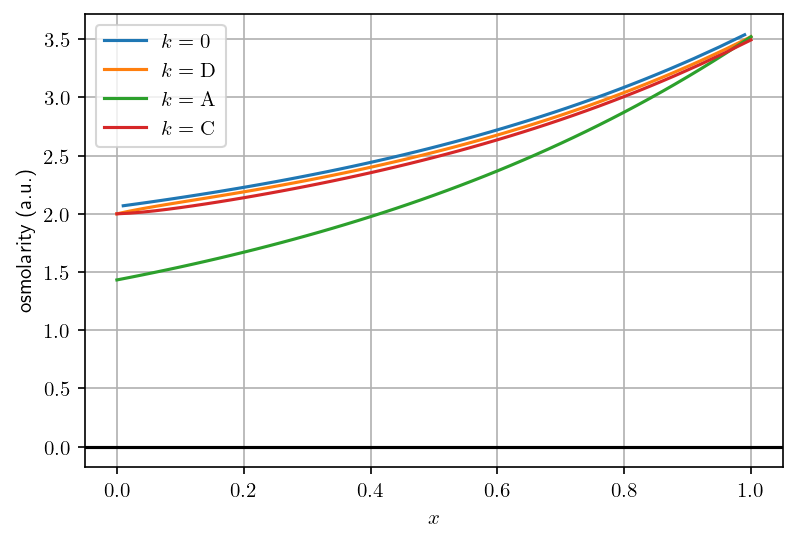
\includegraphics[width=\linewidth]{../results/7-20-2023/osm_high_solute_perm.png}
            \caption{$\gamma_u = \gamma_s = 1.2$}
            \label{fig:high_sol_perm}
        \end{subfigure}
        \caption{$\zeta_\mathrm{D} = \zeta_\mathrm{C} = 10$, $S = 1$, $U = 2$, $C = 2$}
        \label{fig:typical_sol}
    \end{figure}
\end{frame}

\begin{frame}
    \begin{figure}
    \centering
    \begin{subfigure}{0.4\textwidth}
        \centering
        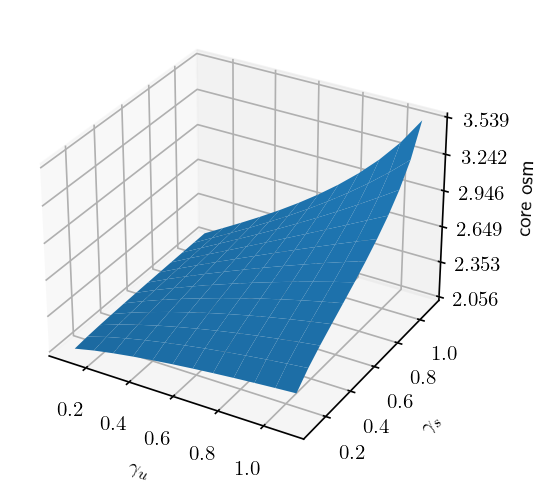
\includegraphics[width=\linewidth]{../results/7-20-2023/core_osm.png}
        \caption{papillary core osmolarity}
        \label{fig:core_osm}
    \end{subfigure}%
    \begin{subfigure}{0.4\textwidth}
        \centering
        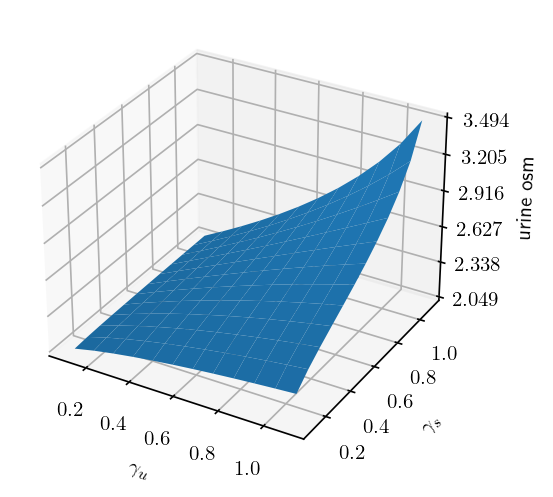
\includegraphics[width=\linewidth]{../results/7-20-2023/urine_osm.png}
        \caption{urine osmolarity}
        \label{fig:urine_osm}
    \end{subfigure}
    \begin{subfigure}{0.4\textwidth}
        \centering
        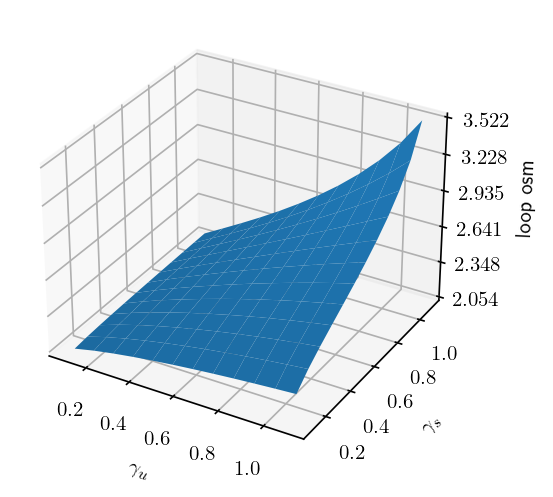
\includegraphics[width=\linewidth]{../results/7-20-2023/loop_osm.png}
        \caption{osmolarity at the turning of Henle's loop}
        \label{fig:loop_osm}
    \end{subfigure}
    \caption{$\zeta_\mathrm{D} = \zeta_\mathrm{C} = 10$, $S = 1$, $U = 2$, $C = 2$}
    \label{fig:pap_osm}
\end{figure}
\end{frame}

\begin{frame}
    Conclusion \#1: urea is an `enabler' of salt reabsorption, while both salt and urea act as sources of osmotic drive.
\end{frame}

\begin{frame}{Long-short loop proportion}
    \begin{figure}
        \centering
        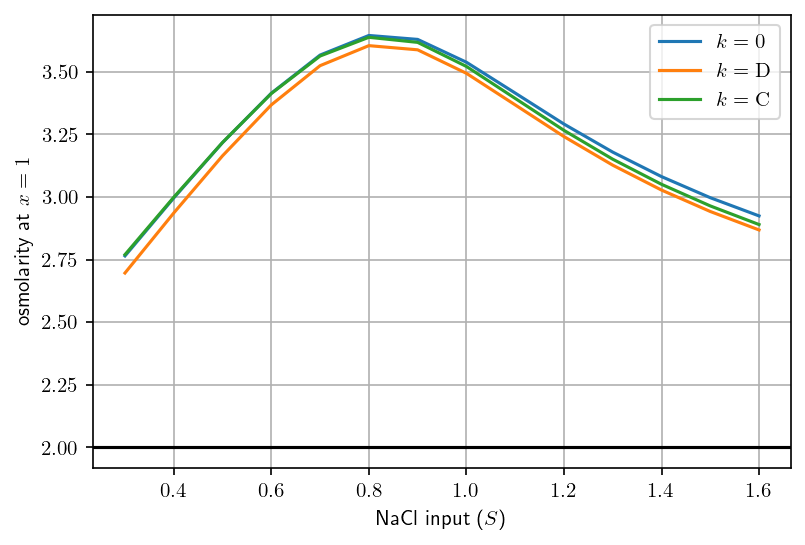
\includegraphics[width=0.8\textwidth]{../results/7-20-2023/osm_loop_fraction.png}
        \caption{$\zeta_\mathrm{D} = \zeta_\mathrm{C} = 10$, $\gamma_u = \gamma_s = 1.2$, $U = 2$, $C = 2$}
        \label{fig:loop_frac}
    \end{figure}
\end{frame}

\begin{frame}[allowframebreaks]
    \bibliographystyle{plainnat}
    \tiny\bibliography{../bibliography}
\end{frame}

\end{document}